\section{UVOD S PREDSTAVITVIJO PROBLEMATIKE, CILJEV IN ZNANSTVENIH VPRAŠANJ}
Populacija je skupina osebkov iste vrste, ki naseljujejo skupni prostor v danem času. Osnovna enota populacije je osebek, ki jih združujemo v deme. Osebki znotraj dema si delijo nekatere genetske značilnosti. Meje populacij navadno niso točno določene, ampak jih uokvirimo raziskovalci iz praktičnih razlogov. Populacijo lahko opišemo s parametri, kot so rodnost, smrtnost, imigracija, emigracija in gostota oz. velikost populacije \citep{krebs_ecology_2001}.

Populacije proučujemo s pomočjo parametrov, na katere vpliva spekter dejavnikov, ki jih lahko delimo na biotske in abiotske. Med abiotske dejavnike razvrščamo temperaturo, vlažnost, pH ipd. Merjenje teh dejavnikov je kdaj enostavno, drugič pa mikrohabitati ekstremno spremenijo razmere in zakrijejo prave vrednosti \citep{cockburn_microhabitat_1983}. Zelo pomembni, a včasih spregledani, pa so tudi biotski dejavniki, h katerim štejemo druge organizme, ki lahko pripadajo isti ali drugi vrsti \citep{krebs_ecology_2001}. Druge vrste lahko očitno vplivajo na populacijske parametre prek npr. kompeticije ali plenjenja, interakcije med osebki iste vrste pa so včasih zabrisane in jih zaznamo šele, ko sistem pogledamo bolj podrobno \citep{lustrik_coexistence_2011}.

Za namen proučevanja lahko razdelimo populacijo na posamezne strukturne enote. Te enote lahko sestavljajo osebki, ki pripadajo istemu spolu, spadajo v isti starostni razred, so v istem razvojnem stadiju, so reproduktivno aktivni ipd. Te dejavnike proučuje populacijska ekologija z namenom boljšega razumevanja vpliva dejavnikov na parametre populacije \citep{krebs_ecology_2001}. V tem delu bi še posebno izpostavili parameter velikosti populacije.

Velikost populacije predstavlja število osebkov oz. število potencialno reproduktivnih enot. Od velikosti populacije in drugih dejavnikov je odvisen njen dolgoročen obstoj. Če je populacija premajhna, lahko zaradi (kombinacije) parjenja v sorodstvu in stohastičnih dogodkov pride do sesutja populacije \citep{amos_when_2001}. V drugem skrajnem primeru, ko je velikost populacije večja od velikosti, ki jo okolje še lahko prenaša, pa pride do sesutja zaradi npr. pomanjkanja hrane v ekstremnih obdobjih \citep{klein_introduction_1968}. V praksi so slednji primeri prostoživečih populacij verjetno relativno redki, saj se je skozi čas vzpostavil mehanizem, ki zagotavlja, da so populacije v dinamičnem ravnovesju z drugimi vrstami in okoljem. Da lahko te pojave proučujemo ali s populacijo upravljamo, je ključnega pomena, da poznamo velikost populacije.

V literaturi je velikost populacije pogosto izpostavljena kot pomemben parameter za proučevanje \citep{kindberg_estimating_2011, chandler_spatially_2013, jimenez_spatial_2017, moqanaki_counting_2018}. Velikost populacije lahko določimo ali ocenimo na različne načine. Omenimo metode lova-ponovnega ulova, ki so med bolj primernimi metodami za oceno številčnosti prostoživečih vrst. Pri teh metodah vzorčimo osebke v časovnem obdobju na določenem območju in v odlovnih intervalih. Osebke zaznamo ali odlovimo, jih označimo in jih nato v naslednjem odlovnem intervalu ponovno zaznamo ali odlovimo ter beležimo, ali so bili že ujeti ali ne. Vsi osebki, ki pridejo v stik z območjem vzorčenja in imajo takrat nezanemarljivo možnost, da jih ujamemo, predstavljajo superpopulacijo.

Področje metod lova-ponovnega ulova je široko. Za ocenjevanje velikosti populacij so zanimive tiste metode, ki zaradi matematičnih lastnosti delujejo na t. i. zaprtih populacijah. To so populacije, ki se v času bistveno ne spreminjajo, torej ni odseljevanja, doseljevanja, rojstev ali smrti. Ta predpostavka je lahko omejujoča, zato se glede na biološke značilnosti vrste vzorčenje prilagodi z denimo relativno kratkim obdobjem vzorčenja. V primeru vzorčenja na območju, ki ne zajame populacije v celoti, navadno prihaja do prehajanja roba območja vzorčenja v in iz območja. S tem je kršena predpostavka o enaki verjetnosti ulovljivosti osebkov in ocena parametrov je lahko pristranska. To prehajanje roba ima za posledico t. i. učinek roba in je že dolgo znan pojav brez zadovoljivih rešitev.

Dosedanje metode rešujejo posledice učinka roba tako, da analizirajo podatke iz zmanjšanega območja vzorčenja, kar naj bi dalo nepristransko oceno gostote. Drugi modeli omogočajo vključevanje individualne spremenljivke. Na podlagi poznavanja neke statistike, povezane z domačim okolišem, lahko raziskovalci povečajo območje vzorčenja v upanju, da bo ocena gostote manj pristranska. Te mere so povprečni najdaljši premik \citep{wilson_evaluation_1985}, razdalja od centroida vzorčenih točk do roba \citep{whittington_comparison_2015} in druge. Kot imata pomisleke že \citet{whittington_comparison_2015}, so te mere pomanjkljive, ker verjetno ne opišejo v zadostni meri odnosa med domačim okolišem osebka in njegovo prisotnostjo oz. odsotnostjo v času vzorčenja.

V tem delu predlagamo novo mero, za katero menimo, da bo bolje opisala domač okoliš osebka in pripomogla k boljši oceni ulovljivosti in velikosti populacije, razširitvi območja vzorčenja in posledično boljši oceni gostote. Verjamemo, da lahko iz porazdelitve prehojenih razdalj ocenimo dvorazsežno porazdelitev, ki nam bo omogočila izračun prostorske individualne spremenljivke in posledično boljšo oceno populacijske gostote.

\subsection{CILJI DISERTACIJE}
Cilj disertacije je izboljšati računanje gostote populacij, kjer med vzorčenjem prihaja do kršitve predpostavke o zaprtosti populacij oz. enaki ulovljivosti.

Na podlagi razdalj med vzorčenimi točkami osebkov v območju vzorčenja bomo ocenili delež prostora/časa, ki ga osebek prebije znotraj območja vzorčenja. To informacijo bomo vključili v model za zaprte populacije kot individualno spremenljivko.

Ker bomo v modelu, ki upošteva individualno spremenljivko, v modeliranje vključili več informacij, pričakujemo, da bo boljši od tistega, kjer te spremenljivke ne bomo uporabili. Za boljši model bomo smatrali tistega, ki bo imel nižji kriterij AICc.

Z vključitvijo informacije o morebitnem prehajanju roba vzorčenega območja v model bomo izboljšali oceno ulovljivosti, saj bomo v model vključili eno od pomembnih komponent, ki vplivajo na spremenjeno zaznavnost in posledično ulovljivost osebkov. Pričakujemo, da bo model, ki vključuje individualno spremenljivko, uspešno kompenziral spremenjeno ulovljivost zaradi prehoda čez rob območja vzorčenja.

Ocena gostote bo izboljšana na račun boljšega poznavanja velikosti dejanskega prispevka območja osebkov v območje vzorčenja, saj bomo iz gibanja osebkov lahko razbrali, kako so razporejeni v prostoru.

Manjše kršitve predpostavke zaprtosti populacije ne bi smele bistveno vplivati na pristranskost ocene gostote. Pričakujemo, da bo razlika med ocenjeno in dejansko gostoto odvisna od razmerja med površino domačega okoliša in površino vzorčenega območja.

\newpage

\section{PREGLED OBJAV}
\subsection{UČINEK ROBA}
Prehajanje roba vzorčenega območja povzroča kršitev predpostavke o zaprtosti populacije oz. enaki verjetnosti ulovljivosti. Sicer sta to dve ločeni predpostavki, a ima kršenje katere koli za posledico različno, heterogeno, ulovljivost osebkov. Heterogenost ulovljivosti med osebki povzroči, da je ocena velikosti populacije vzorčenega območja lahko pristranska. Vpliv tega pojava smo opazili pri naknadni analizi podatkov, ki smo jih uporabili za oceno številčnosti medvedov v Sloveniji \citep{skrbinsek_lustrik_2018}, saj nekateri osebki prehajajo robove območja vzorčenja čez državno mejo Slovenija-Hrvaška. \citet{kendall_robustness_1999} je pokazal, da je verjetnost ulovljivosti osebkov za populacije, ki prehajajo rob vzorčenega območja, $E(\hat{p}_i) = \tau_i p_i$. $\tau_i$ je verjetnost, da se osebek nahaja znotraj vzorčenega območja, pi pa ulovljivost. Ocena velikosti populacije bo nepristranska, če je $tau_i = 1$. V primeru, da je $tau_i$ manjši od 1, pa bo ocena pristranska na način, da bo ulovljivost nižja. To imenujemo učinek roba \citep{hansson_home_1969, white_capture-recapture_1982, wilson_evaluation_1985} in je v študijah lova-ponovnega ulova nezaželen.

\subsubsection[\bfseries{Poskusi reševanja posledic učinka roba}]{Poskusi reševanja posledic učinka roba}
Učinek roba je že dolgo proučevan problem \citep{efford_density_2004}. Prvič se v literaturi s tem ukvarja \citet{dice_census_1938, dice_methods_1941}, ki predlaga, da se območje vzorčenja poveča za polmer domačega okoliša proučevane vrste. Dosedanje raziskave se osredotočajo predvsem na vzorčenje s pomočjo pasti, nameščenih v obliki mreže ali sita \citep{williams_analysis_2002}. V delih, v katerih se ukvarjajo s popravljanjem učinka roba, navadno uporabljajo vzorčenje na situ \citep{parmenter_small-mammal_2003}. Drugi so predlagali podobne popravke, kot so razširitev območja vzorčenja za povprečni najdaljši premik (MMDM, angl. mean maximum distance moved, \citet{wilson_evaluation_1985}), razdaljo med pastmi, oddaljenost ulova od roba območja vzorčenja \citep{boulanger_sources_2004}, povprečno razdaljo premikanja med pastmi in drugi \citep{miller_brown_1997, boulanger_corrigendum_2001, royle_spatial_2013}. Ti popravki po poročanju nekaterih dajejo dobre obete za izboljšanje ocene parametrov \citep{whittington_comparison_2015}.

Drug možni pristop se razlikuje od prejšnjih po tem, da se oceni, kakšen odstotek časa preživijo posamezniki zunaj oz. znotraj vzorčenega območja. \citet{ivan_using_2013} so to želeli oceniti s pomočjo telemetrije. \citet{royle_spatial_2013} poročajo, da sta \citet{white_chapter_2001} uporabila podoben pristop, kjer sta s pomočjo telemetrije ocenila verjetnost ulovljivosti ($\Psi$) in ocenila gostoto kot $\hat{D} = \frac{\hat{N} \Psi}{A}$, kjer je $A$ območje vzorčenja, $\hat{N}$ pa ocenjena velikost populacije s pomočjo modelov za zaprte populacije. Kritika teh pristopov je, da morajo biti osebki, s pomočjo katerih ocenjujemo $\Psi$, opremljeni s telemetrijskimi ovratnicami reprezentativno glede na njihovo dejansko ulovljivost.

Našteti pristopi k reševanju posledic učinka roba so ad hoc. Gre za rešitve ali poskuse njih, ki so nastale z namenom reševanja praktičnih problemov, s katerimi so se v preteklosti srečevali biologi in drugi raziskovalci naravoslovja. V praksi to pomeni, da nimajo splošne oblike in jih zato ni mogoče nadgraditi \citep{royle_spatial_2013}.

V nekatere modele lahko vključimo spremenljivke na nivoju posameznika. S pomočjo dodatne informacije lahko dodatno pojasnimo razlike v ulovljivosti med osebki ali skupinami osebkov. Z uporabo logistične funkcije je mogoče oceniti verjetnosti ulovljivosti $p$ in ponovne ulovljivosti $c$, kot jih opredeli Hugginsov model \citep{boulanger_corrigendum_2001, boulanger_sources_2004}. Ta pristop predstavlja vmesno pot med modeli, ki prostora ne upoštevajo, in pristopi, ki vgradijo prostorsko komponento neposredno v model.

\subsection{NAŠ PRISTOP K REŠEVANJU POSLEDIC UČINKA ROBA}
Na podlagi preliminarnih analiz podatkov za oceno številčnosti medvedov v Sloveniji leta 2007 (Skrbinšek s sod, (v recenziji)) bomo v tem delu raziskali učinkovitost možnega popravka posledic učinka roba. \citet{boulanger_corrigendum_2001} v modelu za izračun velikosti populacije uporabita mero, ki je povezana z razdaljami premikanja med centroidom domačega okoliša in robom območja vzorčenja. S tem naj bi v modelu upoštevala razliko v ulovljivosti osebkov in izboljšala oceno parametrov. V tem delu predlagamo drugo mero, za katero menimo, da bi lahko bolje opisala gibanje osebka znotraj vzorčenega območja in s tem bolje prispevala k popravku učinka roba.

\begin{figure}[htb]
 \begin{center}
 \scalebox{1.2} % h_length
 {\includegraphics*[width=0.5\linewidth]{../r_koda_slike/figures/kernels_hr.png}}
 \end{center}
 \caption[Vzorčene točke in območje vzorčenja]{Vzorčene točke in območje vzorčenja. Primer pojavljanja treh osebkov in območja vzorčenja (črn krog). Modre pike predstavljajo centroide domačega okoliša, sive točke pa točke, ki so bile generirane s pomočjo dvorazsežne normalne porazdelitve. Modre črte povezujejo točke enake verjetnosti pojavljanja (gostoto) osebka.

 \medskip

 Figure \ref{sli:slika1}: Sampled points and sampling area. Distribution of samples from three individuals within sampling area (black circle). Blue points represent centroid of home range, grey points are realized samples according to a two-dimensional normal distribution. Blue lines connect equal probabilities of occurrence (density) of an individual.}
 \label{sli:slika1}
\end{figure}

Predpostavimo, da imamo območje, kjer se nahajajo osebki in ki je praviloma večje od območja vzorčenja (slika ~\ref{sli:slika1}). Na območju so razporejeni centroidi domačih okolišev osebkov. Vsak osebek ima samo en centroid, okoli katerega se giba. V centroidu domačega okoliša je verjetnost ulovljivosti največja, z oddaljevanjem od njega pa pada (slika ~\ref{sli:slika2}). Gibanje bi tako lahko opisali s simetrično dvorazsežnostno normalno porazdelitvijo ali polnormalno porazdelitvijo $p_{ij} = p_0 exp(-\frac{1}{2 \sigma^2} \cdot d)$ \citep[stran~127]{royle_spatial_2013}, kjer je d razdalja od centroida domačega okoliša osebka do točke ulova, $\sigma^2$ pa varianca, ki je parameter te porazdelitve. Uporabo domačega okoliša si lahko predstavljamo kot zvonec, z vrhom v centroidu. Veliko večino točk pričakujemo na oddaljenosti treh standardnih odklonov od centroida.

\begin{figure}
\centering
\begin{subfigure}{0.5\textwidth}
  \centering
  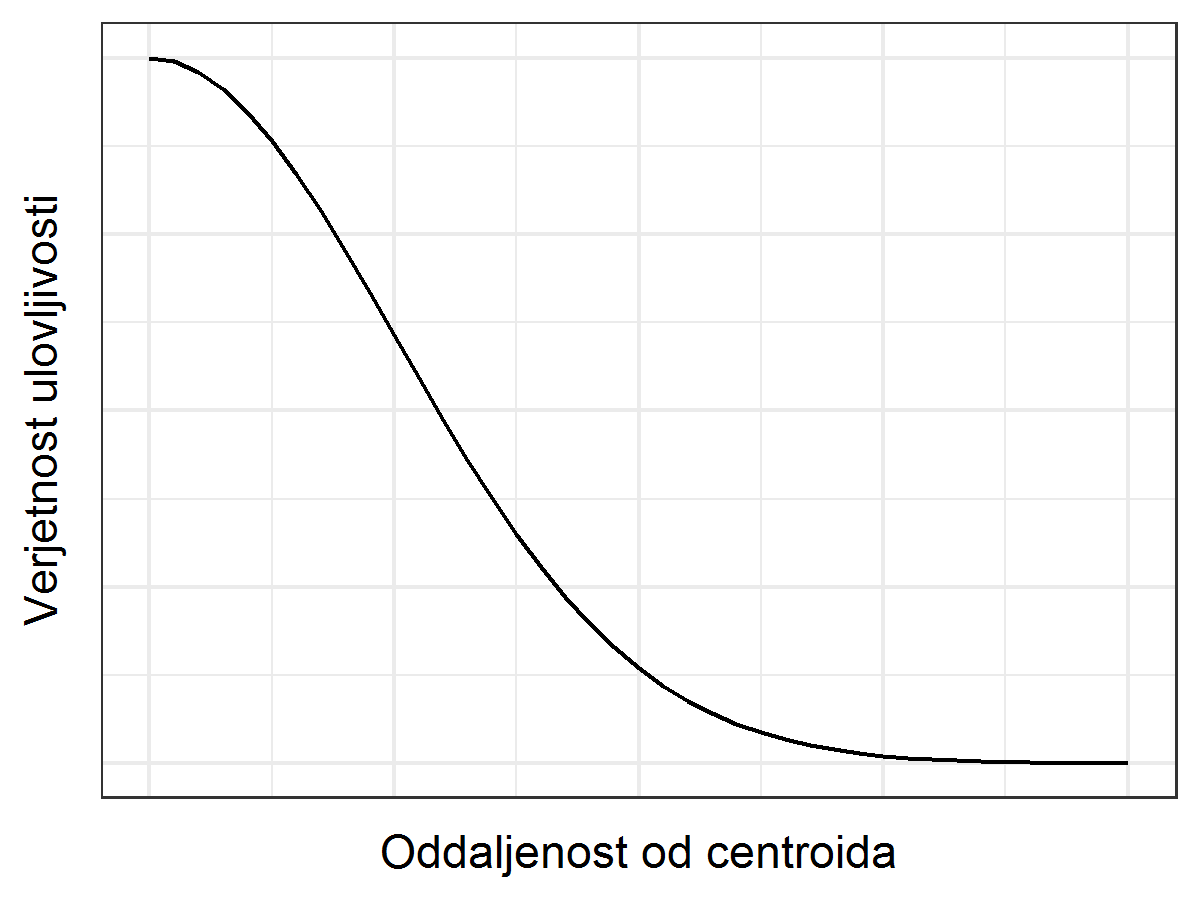
\includegraphics[width=0.9\linewidth]{../r_koda_slike/figures/half_normal.png}
  % \caption{A subfigure}
  \label{sli:sub2.1}
\end{subfigure}%
\begin{subfigure}{0.5\textwidth}
  \centering
  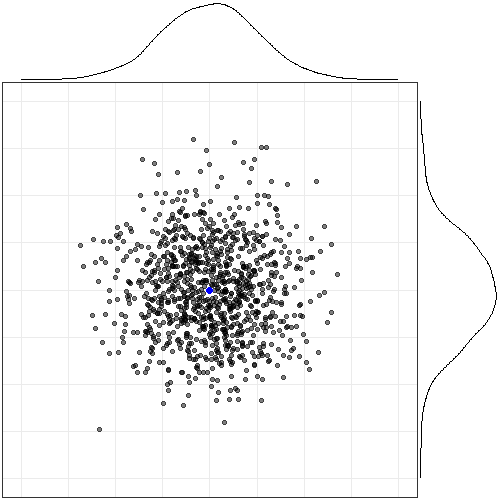
\includegraphics[width=0.9\linewidth]{../r_koda_slike/figures/homerange_usage.png}
  % \caption{A subfigure}
  \label{sli:sub2.2}
\end{subfigure}
\caption[Funkcija simuliranja vzorčnih točk in realizirane točke]{Funkcija simuliranja vzorčnih točk in realizirane točke. Levo je ponazorjena verjetnost pojavljanja osebka glede na polnormalno porazdelitev, ki jo uporabimo za simulirane domačega okoliša. Osebek se bo najpogosteje nahajal okoli izhodišča (levo), z oddaljenostjo od njega pa bo ta verjetnost padala. Prikaz desno ponazarja ``ulov'' osebka (sive pike) v prostoru in realizacijo dvorazsežne normalne porazdelitve. Krivulji ob desni in zgornji stranici sta robni porazdelitvi.

\medskip

Figure \ref{sli:slika2}: Function used for simulation and its realization. Left depicts a half-normal distribution which we use to model home range. Highest probability of occurrence is in the center and decreases with distance from it. Right image shows realization of two-dimensional normal distribution. Density curves above and to the right of the figure margins are marginal distributions.}
\label{sli:slika2}
\end{figure}

Osebkom, ki imajo pretežni delež domačega okoliša znotraj vzorčenega območja, lahko pripišemo delež njihovega domačega okoliša znotraj območja vzorčenja 1. Če se centroid osebka nahaja v bližini roba območja vzorčenja, lahko pričakujemo, da bo del časa osebek preživel zunaj območja. V tem času med vzorčenjem ne bo zaznaven (ulovljiv), zato bo delež njegovega domačega okoliša znotraj območja vzorčenja manjši od 1. Podobno velja za krivulje, ki nimajo parametrične oblike (neparametrične krivulje).

Osebke med premikanjem lovimo ter beležimo lokacijo in čas, ko smo jih zaznali. Točke na sliki \ref{sli:slika2} desno predstavljajo take ulove. Predpostavljamo, da te točke predstavljajo reprezentativno gibanje osebkov. Histogram razdalj med pari točk predstavlja razdalje, ki jih osebek lahko prehodi. To porazdelitev uporabimo pri izračunu deleža, ki pripada okolišu osebka znotraj območja vzorčenja. Delež porazdelitve znotraj območja vzorčenja uporabimo v modelu kot individualno spremenljivko.

\subsection{METODA LOVA-PONOVNEGA ULOVA}
Velikost populacije lahko podamo na dva načina - kot število osebkov na območju vzorčenja ali neposredno kot gostoto (število osebkov na enoto). Zaradi bioloških značilnosti oziroma velikega območja, na katerem se populacija razteza, vseh živali fizično ni mogoče zaznati v izvedljivih časovnih, finančnih in drugih okvirih. Zato moramo poseči po pristopih, ki omogočajo, da zaznanim osebkom prištejemo tiste, ki smo jih spregledali. Na ta način lahko ocenimo vsoto zaznanega in pričakovanega dela populacije. S pomočjo znanstveno preverljivih metod lahko oceni podamo interval zaupanja, s katerim lahko sporočimo tudi, kako natančna je naša ocena.

Ko na določenem območju z gotovostjo zaznamo vse osebke, jih preprosto preštejemo. To imenujemo cenzus, kjer predpostavimo, da vse osebke zagotovo zaznamo ($p=1$). Cenzusi v ekologiji niso pogosti, ker določenega deleža osebkov običajno ni mogoče zaznati. Metode, ki upoštevajo dejstvo, da vsi osebki med vzorčenjem niso zaznani s popolno gotovostjo ($p < 1$), so osnovane na podlagi štetja na ploskvah, oddaljenosti od opazovalca ter lova-ponovnega ulova \citep{williams_analysis_2002}.

Metoda štetja na ploskvah deluje na način, da območje, kjer želimo oceniti številčnost neke populacije, razdelimo na prostorske podenote. Na vzorcu podenot izvedemo vzorčenje in iz ocen številčnosti v podenotah sklepamo o številčnosti na večjem območju. Pri tem moramo upoštevati več predpostavk, saj ima sklepanje z vzorca na večje območje več pasti \citep{williams_analysis_2002}.

Metode, kjer se beleži oddaljenost osebka od točke opazovanja, v prvi vrsti podajo oceno gostote. Opazovanje lahko poteka na naključno izbranih točkah ali transektih, vhodni podatek za računanje pa je razdalja osebka do transekta. Predpostavlja se, da je na transektih, ki jih popisovalec pregleduje, zaznavnost 1, z oddaljenostjo od transekta pa zaznavnost pada po krivulji. Tip krivulje lahko izberemo na podlagi teorije ali prakse \citep{williams_analysis_2002}.

Do sedaj opisani načini za oceno številčnosti ne upoštevajo identitete zaznanega osebka, kar je domena metod lova-ponovnega ulova.

\subsubsection[\bfseries Osnovne značilnosti metode lova-ponovnega ulova]{Osnovne značilnosti metode lova-ponovnega ulova}
Metode lova-ponovnega ulova se od zgoraj naštetih metod razlikujejo po tem, da kot informacijo uporabljajo identiteto osebka. Zanesljiva določitev identitete osebka je najvišja kvaliteta podatka, ki ga lahko pridobimo za oceno številčnosti populacije. Kljub temu da so bile nekatere matematične osnove metode lova-ponovnega ulova razvite že pred več stoletji, se je paleta modelov razširila in prešla v splošno uporabo v začetku dvajsetega stoletja \citep{pollock_capture-recapture_2000}.

Poznamo več matematičnih modelov in vsak ima svoje prednosti in slabosti. V eni od delitev lahko modele razvrstimo v dve večji skupini, ki se razlikujeta po tem, da so primerni za odprte oz. zaprte populacije. O odprtih populacijah govorimo takrat, ko osebki med vzorčenjem prihajajo in odhajajo iz populacije. Zaprte populacije tega prehoda ne predpostavljajo in je zato že v osnovi pojem ``velikost populacije'' lažje opredeliti. Pregled metod za zaprte populacije v svojem klasičnem delu opišejo \citet{otis_statistical_1978}, kasneje pa še drugi (tudi za odprte), kot so \citet{white_capture-recapture_1982}, \citet{seber_review_1986} in \citet{white_program_1999}.

\subsubsubsection{Prepoznavanje osebkov}
Da lahko osebek prepoznamo kot edinstvenega, ga moramo nekako ujeti oz. zaznati. V preteklosti je to predstavljalo fizičen ulov, nakar so žival nedvoumno označili. Osebke se označuje na načine, da je oznaka trajna ali začasna (npr. označevanje robnih lusk ščita pri želvah \citep{pike2005}, ščipanje ušes ali nohtov pri manjših sesalcih \citep{wiewel_assessing_2007}, pisanje številk na krila metuljev \citep{jugovic_movement_2017}, ščipanje prstov pri dvoživkah \citep{campbell_evaluation_2009}, opremljanje z ušesnimi značkami, barvanje kožuha, tetoviranje...).

Z napredovanjem molekularnih tehnik in večanjem računalniške moči je danes možen “ulov” brez fizičnega stika z osebki. Tako je manj verjetno verjetno, da bo osebek spremenil vedenje in s tem svojo ulovljivost. V praksi to pomeni, da iz neinvazivno nabranih vzorcev (brez stika s preiskovanim osebkom, npr. iz sluzi, sline, dlake, iztrebka, perja) preko genotipizacije DNK z visoko zanesljivostjo določimo identiteto osebka \citep{waits_noninvasive_2005}. Tak genotipiziran vzorec štejemo za “ulov” osebka. Drug pristop lahko uporabimo pri živalih, ki imajo značilno obarvano kožo ali dlako (npr. trebuh nekaterih dvoživk, obarvanost kožuha pri risu), kjer lahko s pomočjo fotografij in računalniških programov razločimo med osebki.

\subsubsubsection{Območje vzorčenja}
Ulov in označevanje osebkov potekata na geografsko določenem območju, ki za živali z velikim območjem gibanja pogosto le deloma zaobjame proučevano populacijo. Velikost območja vzorčenja je navadno omejena zaradi velikih razdalj potovanj, s fizičnimi mejami (otoki) ali pa s političnimi mejami (parkov, držav ali drugih administrativnih enot). Iz tega sledi, da ko osebke zaznavamo (lovimo), njihovo gibanje ni nujno omejeno na naše arbitrarno določeno območje vzorčenja.

\subsubsubsection{Domač okoliš}
Območje domačega okoliša osebka predstavlja prostor, kjer se zadržuje osebek med dnevnimi aktivnostmi. Raba prostora navadno sovpada s trenutnimi potrebami osebkov (iskanje hrane, partnerjev) in se v času lahko spreminja. Velikost območja je odvisna od velikosti organizma, bioloških značilnosti vrste, topografije, znotrajvrstnih in medvrstnih interakcij ter razpoložljivosti hrane in drugih virov, potrebnih za življenje.

\subsubsubsection{Superpopulacija}
Populacijo opredeljujemo kot skupino osebkov, ki se nahajajo znotraj območja vzorčenja. Poleg osebkov, ki se neprestano zadržujejo znotraj območja vzorčenja, lahko zaznamo tudi osebke, ki prehajajo njegove meje, ker se njihov domač okoliš le deloma prekriva z našim arbitrarnim območjem vzorčenja. Njihova zaznavnost je v povprečju nižja od osebkov, ki se v prostoru in času stalno nahajajo v območju vzorčenja. Skupaj z ostalimi osebki tvorijo t. i. superpopulacijo, za katero pa ne vemo natančno, kako je prostorsko omejena.

\subsection{PREDPOSTAVKE METOD LOVA-PONOVNEGA ULOVA}
Kot velja za vse modele, tudi pri modelih lova-ponovnega ulova veljajo nekatere predpostavke. Njihova kršitev ima lahko blage ali hude posledice. V splošnem se trudimo, da predpostavkam zadostimo. V primerih simuliranih vrednosti lahko nekatere predpostavke zanemarimo ali pa jih nadzorujemo, kar nam pomaga proučevati, kaj se dogaja pri njihovem kršenju.

\subsubsection[\bfseries Zanesljivost označevanja]{Zanesljivost označevanja}
Da osebek nedvoumno in zanesljivo označimo pomeni, da se oznaka v prostoru in času ne izgubi ali spremeni in da jo raziskovalec lahko zanesljivo prebere. V preteklosti se je uporabljalo neposredne načine označevanja (ušesne oznake, tetovaže, rezanje uhljev, barvanje krempljev …), danes pa se vsaj za nekatere skupine živali (npr. večji sesalci) uporablja pristope, temelječe na molekularni genetiki. Ker za nabiranje nekaterih tipov vzorcev (iztrebkov, dlak, peres) ne potrebujemo neposrednega stika z osebkom in pri nabiranju ne motimo vedenja, to imenujemo neinvazivno vzorčenje. Pri genetskem vzorcu je zaradi napak genotipizacije ali identičnih dvojčkov mogoče, da genotip določimo narobe, vendar so metode, če so pravilno uporabljene, kljub temu zelo zanesljive v smislu označevanja osebkov \citep{waits_noninvasive_2005}. Za živali, ki imajo značilne vzorce kožuha, se lahko uporablja posnetke s samodejnih foto pasti, ki so doživele razmah uporabe v zadnjih desetih letih \citep{oconnell_camera_2010}.

\subsubsection[\bfseries Enaka ulovljivost]{Enaka ulovljivost}
Predpostavlja se, da imajo vse živali znotraj območja vzorčenja enako verjetnost, da jih bomo zaznali oz. ulovili v danem odlovnem intervalu. Do neenake ulovljivosti lahko pride zaradi več vzrokov. Če imajo živali različne ulovljivosti, govorimo o heterogenosti ulovljivosti. Zvišanje (t. i. \textit{trap-happy}) ali znižanje ulovljivosti (t. i. \textit{trap-shy}) je posledica pristranskega vzorčenja, bodisi zaradi opazovalca ali proučevanega subjekta \citep{roche_recapture_2013}. Do heterogenosti ulovljivosti lahko pride tudi v primerih, ko območje vzorčenja geografsko ni zaprto, osebki pa prehajajo iz in v območje vzorčenja. Avtorji opozarjajo, da kršenje te predpostavke vpliva na pristranskost cenilke velikosti populacije. Smer pristranskosti je znana. Ko je ulovljivost podcenjena, je ocena velikosti populacije precenjena. Če ulovljivost precenimo, je ocena velikosti populacije podcenjena \citep{williams_analysis_2002}.

Heterogenost ulovljivosti lahko testiramo s pomočjo informacijsko-teoretičnega pristopa \citep{burnham_model_2002}. Podatke analiziramo s pomočjo različnih parametrizacij modela. V osnovnem modelu predpostavimo enako ulovljivost, v drugih pa upoštevamo heterogenost ulovljivosti, ki jo sumimo (npr. na račun privabljanja ali odbijanja od pasti, prehajanja roba območja vzorčenja). Modele sortiramo po velikosti statistike AICc. Če je zaznati heterogenost ulovljivosti, bo imel osnovni model, ki predpostavlja enako ulovljivost, znatno višjo vrednost AICc od ostalih. Ista avtorja na strani 70 podajata okvirne vrednosti razlik med modeli. Razlike v razponu med 0 in 2 so v zmerno podporo modelu z nižjo vrednostjo AICc, od 4 do 7 v znatno podporo, razlike nad 10 pa lahko smatramo kot ključno podporo v prid modela z nižjim AICc.

\subsubsection[\bfseries Zaprtost populacije]{Zaprtost populacije}
Demografsko zaprta populacija je tista, pri kateri v času vzorčenja ne prihaja do sprememb v smislu emigriranja, imigriranja, rojstev ali smrti. Populacija se torej strukturno ne spreminja. Z nekaterimi metodološkimi pristopi lahko vsaj za nekatere dolgožive vrste zagotovimo, da je kršenje predpostavke v smislu rojstev ali smrti minimalno. V prispevku, kjer smo ocenili velikost populacije rjavega medveda v Sloveniji, smo izbrali obdobje vzorčenja jesen, ko smo prepričani, da ne prihaja do poleganja mladičev (Skrbinšek s sod. (v recenziji)). Osebke, ki so dokumentirano izgubljeni iz populacije v času vzorčenja, lahko naknadno prištejemo končni oceni. Ker imajo nekatere vrste relativno velika območja gibanja, je zagotavljanje vzorčenja na dovolj velikem območju težavno. V takih primerih lahko upoštevamo heterogenost ulovljivosti in uporabimo, če je možno, več virov informacij \citep{boulanger_multiple_2008}.

Za to predpostavko obstajajo testi, kot so jih predlagali \citet{otis_statistical_1978} in \citet{stanley_closure_1999}. Teste pesti preobčutljivost ali pa prenizka moč, da zaznajo nekatere tipe zaprtosti populacije. Modeli za zaprte populacije lahko predvidevajo heterogenost ulovljivosti, vedenjski odziv ali spremembo ulovljivosti v času \citep{otis_statistical_1978}, zaradi česar so lahko kljub učinku roba uporabni v smislu, da niso pristranski. Kljub temu pa prehajanje lahko zmanjša ulovljivost do te mere, da je parametre modela težko oceniti oz. so nesmiselni (npr. interval zaupanja od $-\infty$ do $\infty$). Pri organizmih, ki imajo že zaradi svojih bioloških značilnosti nizko zaznavnost (npr. ris), je to lahko za raziskavo pogubno.

\subsection{CENILKA VELIKOSTI POPULACIJE ZA DVA ODLOVNA INTERVALA}
Cenilko za velikost populacije, ko vzorčimo v dveh odlovnih intervalih, imenujemo Lincoln-Petersenova cenilka. Ime je dobila po Lincolnu in Petersenu, ki sta jo uporabila pri svojem delu, vendar nista avtorja \citep{williams_analysis_2002}. Pred njima jo je uporabil že vsaj Laplace, ko je v 18. stoletju ocenil število prebivalcev Pariza. Lincoln-Petersonovo cenilko je mogoče izpeljati na več načinov, spodaj pa bomo predstavili le enega, ker se navezuje na Hugginsov model za zaprte populacije, ki ga uporabimo v tej raziskavi.

Pri ulovu nedvoumno označimo osebke in jih spustimo, hkrati pa zabeležimo vse že prej označene osebke. Lovno zgodovino si lahko predstavljamo kot matriko velikosti n $\times$ m. Vrstice predstavljajo osebke, stolpci pa odlovne intervale. V primeru ulova in prepoznavanje osebka v določenem odlovnem intervalu je vrednost matrike na tem mestu 1, sicer pa 0. Spodnja matrika prikazuje tri osebke, ki so bili ujeti v dveh odlovnih intervalih. Prvi osebek je bil ujet (in označen) samo v prvem intervalu, drugi osebek samo v zadnjem, tretji osebek pa je bil zabeležen v obeh odlovnih intervalih.

\[
M = \begin{bmatrix}
1&0\\
0 & 1 \\
1 & 1
\end{bmatrix}
\]

Lincoln-Petersenova cenilka \citep{williams_analysis_2002} je prirejena za dva odlovna intervala in temelji na razmerju med številom ujetih živali v prvem intervalu ($n_1$) in populacijo ($N$) ter razmerju med številom ujetih živali v obeh intervalih ($m_2$) in številom živali, ujetih v drugem intervalu ($n_2$).

\[
\frac{n_1}{N} = \frac{m_2}{n_2}
\]

in če izpostavimo N, dobimo cenilko

\[
\hat{N} = \frac{n_1 n_2}{m_2}.
\]

V primeru, da imamo dva odlovna intervala, je verjetnost ulovljivosti $p^{*}$ produkt verjetnosti ulovljivosti v prvem ($p_1$) in drugem ($p_2$) odlovnem intervalu z naslednjo enakostjo

\[
p^* = 1 - (1-p_1)(1-p_2).
\]

Parameter $\hat{p}^{*}$ lahko izrazimo tudi s pomočjo pogojnega multinomskega modela

\[
P(x_{ij} \mid r, p_1, p_2) = \frac{r!}{x_{11}! x_{10}! x_{01}!} \cdot \Big(\frac{p_1 p_2}{\hat{p}^{*}}\Big)^{x_{11}} \Big(\frac{p_1 q_2}{\hat{p}^{*}}\Big)^{x_{10}} \Big(\frac{q_1 p_2}{\hat{p}^{*}}\Big)^{x_{01}},
\]

kjer je $r$ unikatno število ujetih živali. Tako dobimo oceno parametrov največjega verjetja


\[
\hat{p}_1 = \frac{x_{11}}{x_{11} + x_{01}}
\]

ter

\[
\hat{p}_2 = \frac{x_{11}}{x_{11} + x_{10}}.
\]

S tem lahko izrazimo $p^{*}$

\begin{align*}
p^* &= 1 - (1-\hat{p}_1)(1-\hat{p}_2) \\[5pt]
    &= \frac{r x_{11}}{(x_{11} + x_{10})(x_{11} + x_{01})},
\end{align*}

ki ga lahko uporabimo v kanonični cenilki za $\hat{N}$

\[
\hat{N} = \frac{r}{\hat{p}^{*}} = \frac{(x_{11} + x_{10})(x_{11} + x_{01})}{x_{11}} = \frac{n_1 n_2}{m_2}
\]
\[
\hat{N} = \frac{(n_1 + 1)(n_2 + 1)}{m_2 + 1} - 1.
\]

Varianca za $\hat{N}$ je $[(n_1 + 1)(n_2 + 1)(n_1 - m_2)(n_2 - m_2)]/[(m_2 + 1)(m_2 + 2)]$, interval zaupanja pa je mogoče izpeljati na različne načine \citep{williams_analysis_2002}.

Za modeliranje heterogenosti ulovljivosti so razvili model $M_h$ \citep{otis_statistical_1978}

\[
P(f_1, \ldots f_K \mid F) = \frac{N!}{\big(\prod_{j=1}^{K} f_j !\big)\big(N - M_{K+1}\big)} \pi_{0}^N-M_{K+1} \prod_{j=1}^{K} \pi_{j}^{f_j},
\]

kjer je parameter $\pi_j = \int_{0}^{1} \frac{K!}{(K-j)!j!} p^j (1-p)^{K-j} dF(p)$.


\subsubsection[\bfseries Hugginsov model za zaprte populacije]{Hugginsov model za zaprte populacije}
Primer za dva odlovna intervala zgoraj lahko posplošimo na poljubno število. Eno takih posplošitev najdemo v modelu Huggins-Alho (znan tudi kot Hugginsov model, kot ga imenujemo tudi v tem delu, \citet{huggins_statistical_1989}). Ta model omogoča, da ocenimo velikost populacije, pri tem pa lahko upoštevamo tudi razlike v verjetnosti ulovljivosti ($M_h$) s pomočjo individualne spremenljivke. Pogojna verjetnostna funkcija je

\[
L = \prod_{i=1}^{n} \prod_{j=1}^{t} p_{ij}^{I_{ij}} (1 - p_{ij})^{(1 - {I_{ij}})}.
\]

Ključni dodatek je ocena ulovljivosti z uporabo spremenljivk na nivoju posameznika za vsak odlovni interval s pomočjo že prej omenjene logistične funkcije

\[
p_{ij} = \frac{e^{b_0 + \beta_1 z_i \beta_2 x_j \alpha z_{ij}}}{1 + e^{b_0 + \beta_1 z_i \beta_2 x_j \alpha z_{ij}}},
\]

kjer je $z_i$ vektor individualnih spremenljivk (npr. delež časa, ki ga osebek preživi znotraj območja vzorčenja), $x_j$ vektor okoljskih spremenljivk, kot je denimo količina padavin, $z_{ij}$ pa predstavlja spremenljivo, ki spremeni ulovljivost v času. Tako lahko s pomočjo individualne spremenljivke upoštevamo, da imajo osebki različno ulovljivost. \citet{akanda_estimation_2014} sta za izračun $p_{ij}$ uporabila še GLM, GEE in GLMM.

Hugginsov model, za razliko od npr. \citet{pollock_use_1984}, ne vsebuje parametra za velikost populacije $\hat{N}$, zato lahko $p_i$ ocenimo s pomočjo zveznih spremenljivk. Cenilka za velikost populacije je

\[
\hat{N}(\theta) = \sum_{i=1}^{N} \frac{1}{p_{i}(\theta)},
\]

kjer predpostavimo, da je $\theta$ že znana. Parameter $p_i$ definiramo kot verjetnost, da smo osebek ulovili vsaj v enem odlovnem intervalu

\[
p_i(\theta) = P(C_i) = 1 - \prod_{j=1}^{K}(1-\hat{p}_{ij}).
\]

Nepristranska cenilka variance ($\hat{\nu}(\theta)$) je

\[
s^2 = \sum_{i=1}^{N} p_{i}^{-2} (\theta)(1-p_i (\theta)).
\]

\subsection{MODEL CAPWIRE}
Modeli paketa CAPWIRE \citep{miller_new_2005} gradijo na osnovi modelov z mešano ulovljivostjo. Za vhodne podatke uporabi skupno število ulovov posameznega osebka, ne glede na število odlovnih intervalov ali koliko vzorcev je bilo nabranih v posameznem intervalu. Modele parametra oceni s pomočjo multinomske porazdelitve.

Na voljo sta dva modela, ECM in TIRM. Prvi predpostavlja, da imajo vsi osebki enako verjetnost, da so zaznani. Model TIRM pa predpostavlja, da obstajata dve skupini osebkov, ki imata dve različni ulovljivosti. Skupino modelov, ki predpostavljajo več skupin, imenujemo modeli mešane ulovljivosti.

\subsection{SIMULACIJE KOT ORODJE ZA RAZISKOVANJE}
V matematičnih modelih opišemo pojav s funkcijami, ki so lahko preproste ali kompleksne. S kompleksnostjo pojava narašča tudi kompleksnost funkcij. Drug pristop je opis pojava s stohastičnimi procesi - simulacijami. Pojav razdelimo na manjše podenote in vsako enoto simuliramo kot samostojni proces. Razpon vrednosti, ki jih zavzemajo parametri podenote, določi raziskovalec, najpogosteje na podlagi teoretskih osnov in poznavanja pojava. Podenota ni samostojna, ampak je odvisna od drugih podenot in parametrov, ki jih določi raziskovalec. V ekologiji lahko na tak način simuliramo gibanje in obnašanje živali ter proučujemo interakcijo med osebki oz. višjimi enotami in okoljem \citep{bolker_ecological_2008}.
